\section{Rezultati simulacija}\label{sec:simulacije}

\subsection{Postavke}

Parametri su ilustrativni i ne opisuju određenu vrstu: $\pAm=100$~J\,d$^{-1}$\,cm$^{-2}$, $\pM=20$~J\,d$^{-1}$\,cm$^{-3}$, $\EG=5000$~J\,cm$^{-3}$, $\beta_S=4$, $\beta_R=1$, $\beta_E=5$~cm\,d$^{-1}$, $k_E=0{,}01$, $f=1$, $L_0=0{,}3$~cm. Odatle slijede $\kappa=0{,}8$ i $L_\infty=4$~cm, a $\Vref=(2~\text{cm})^3$. Kod je u \texttt{docs/alpha-handbook/sim/}.

\paragraph{Zašto $k_E=0{,}01$.} U ravnoteži spremišta vrijedi $E_T=k_E E_E$ (jedn.~\eqref{eq:mE}), pa je $k_E$ omjer energije u transportu i energije u spremištu. Red veličine tog omjera procjenjujemo za čovjeka, kao najbolje dokumentiranu referentnu životinju. Pretpostavljeno tijelo je muškarac od 70~kg i 1,75~m, a energijska vrijednost lipida $39$~kJ\,g$^{-1}$, kao u Koraku 3 (pogl.~\ref{sec:protokol}).
\begin{itemize}
\item \textbf{Volumen plazme:} 44~$\pm$~5~mL\,kg$^{-1}$ u 23 zdrava ispitanika (Haller i sur. 1992) \pouzd{sažetak}, dakle $\approx3{,}1$~L.
\item \textbf{Trigliceridi u plazmi:} 100~$\pm$~21~mg\,dL$^{-1}$ natašte i 237~$\pm$~40~mg\,dL$^{-1}$ tijekom stalnog unosa masti (Park i sur. 2000) \pouzd{sažetak}. To je 3,1–7,3~g, odnosno 0,12–0,28~MJ \pouzd{izvedeno}.
\item \textbf{Glukoza i slobodne masne kiseline:} uz \emph{pretpostavljene} koncentracije od 5~mmol\,L$^{-1}$ glukoze (16~kJ\,g$^{-1}$) i do 1~mmol\,L$^{-1}$ slobodnih masnih kiselina (≈270~g\,mol$^{-1}$, 39~kJ\,g$^{-1}$) sadrže još $\approx0{,}04$ i $\approx0{,}03$~MJ.
\item \textbf{Masno tkivo:} kod muškaraca normalne uhranjenosti masa masti izmjerena DXA-om iznosi 3–6~kg po m$^2$ visine (referentne vrijednosti NHANES; Kelly, Wilson i Heymsfield 2009) \pouzd{puni tekst}. Za visinu od 1,75~m to je 9–18~kg. Donja granica, 9~kg, sadrži $\approx360$~MJ \pouzd{izvedeno}.
\end{itemize}
Gornja procjena omjera je $(0{,}28+0{,}04+0{,}03)/360\approx1\times10^{-3}$, a uz trigliceride natašte $\approx5\times10^{-4}$. Uz 18~kg masti omjer se još prepolovi. Stvarni $k_E$ je dakle oko $10^{-3}$ ili manji, pa je $k_E=0{,}01$ konzervativna gornja granica s rezervom od reda veličine. Simulacije transportu pridaju veću zalihu nego što je realno, pa pretpostavka (ii) iz pogl.~\ref{sec:propozicije} kod stvarnih organizama vrijedi s još većom rezervom.

\subsection{S1 · Rast ne razlikuje $\alpha$, spremište razlikuje}

\begin{figure}[ht]
\centering
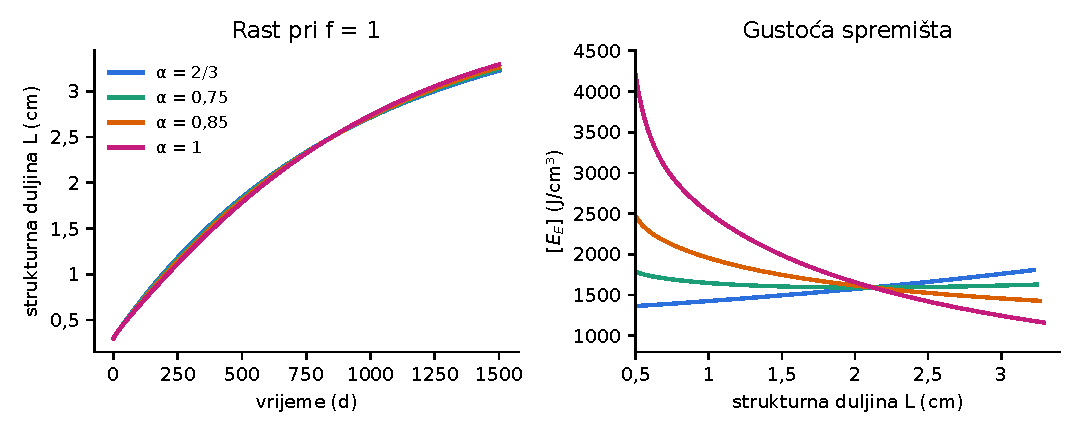
\includegraphics[width=\linewidth]{figures/fig_rast_spremiste.pdf}
\caption{Lijevo: krivulje rasta za četiri vrijednosti $\alpha$ uz iste ostale parametre. Desno: gustoća spremišta po strukturi prema strukturnoj duljini.}
\label{fig:rast}
\end{figure}

Krivulje rasta za $\alpha=2/3$ i $\alpha=1$ razlikuju se najviše oko \GrowthMaxDiff~\% (tablica~\ref{tab:rast}), a gustoća spremišta mijenja se kvalitativno. Uz $\alpha=1$ mladi su deblji od starih, a uz $\alpha=2/3$ tanji. To je numerička potvrda H7: gustoća spremišta mladih i odraslih nosi informaciju o $\alpha$, a krivulja rasta gotovo ne nosi (P1, P2).

\begin{table}[ht]
\centering\small
\caption{Rast i gustoća spremišta ($[E_E]$ u J\,cm$^{-3}$) za četiri vrijednosti $\alpha$. Nagib je $d\log[E_E]/d\log V$ za $1<L<3{,}5$~cm. „P2“ je kvazi-ravnotežno predviđanje $2/3-\alpha$. „Naivni $\alpha$“ je $2/3-\text{nagib}$, a pristranost je naivni $\alpha$ umanjen za istinski.}
\label{tab:rast}
\begin{tabular}{@{}ccccccrrrr@{}}
\toprule
$\alpha$ & $L(200)$ & $L(600)$ & $L(1500)$ & $[E_E]_{L=1}$ & $[E_E]_{L=3}$ & nagib & P2 & naivni $\alpha$ & pristranost \\
\midrule
\inputtab figures/tables/tab_growth.tex
\bottomrule
\end{tabular}
\end{table}

\subsection{S2 · Profil vjerodostojnosti}

Iz modela s $\alpha=0{,}75$ generirani su sintetski podaci: 25 mjerenja duljine s 2~\% šuma i, u drugoj varijanti, još 8 mjerenja $[E_E]$ s 10~\% šuma. Za svaki fiksirani $\alpha$ na mreži 0,50–1,00 (korak 0,025) ostali su parametri ponovno fitani ($\pAm$, $\pM$, $\beta_S$, a za drugu varijantu i $k_E$).

\begin{figure}[ht]
\centering
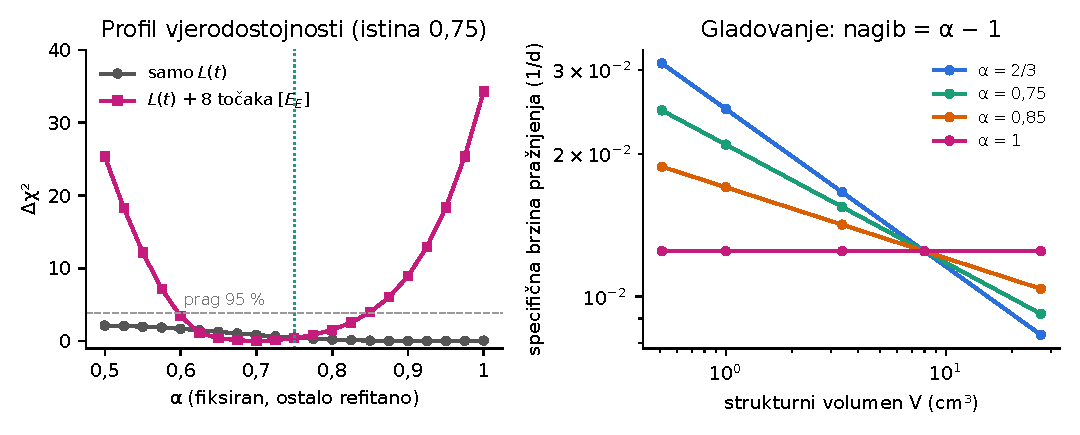
\includegraphics[width=\linewidth]{figures/fig_profil_gladovanje.pdf}
\caption{Lijevo: profil vjerodostojnosti za $\alpha$ (istinski $\alpha=0{,}75$, točkasta crta); isprekidana crta je prag 95~\% ($\Delta\chi^2=3{,}84$). Desno: specifična brzina pražnjenja spremišta pri gladovanju prema strukturnom volumenu (log–log); nagib je $\alpha-1$.}
\label{fig:profil}
\end{figure}

\begin{itemize}
\item \textbf{Samo $L(t)$:} $\Delta\chi^2\le\ProfLonlyMax$ na cijelom rasponu 0,50–1,00. Interval pouzdanosti obuhvaća cijeli raspon, pa $\alpha$ \emph{nije} identifikabilan.
\item \textbf{$L(t)$ + 8 točaka $[E_E]$:} 95~\% interval pouzdanosti seže od \CIlo{} do \CIhi{} (najbolja vrijednost na mreži \AlphaBestProf; istina 0,75). Obje granice leže unutar mreže. Profil je asimetričan: prema nižim vrijednostima raste sporije ($\Delta\chi^2=3{,}4$ pri $\alpha=0{,}60$, $25$ pri $0{,}50$), a prema višima strmo ($\Delta\chi^2\ge8{,}9$ za $\alpha\ge0{,}9$).
\end{itemize}

\subsection{S3 · Gladovanje: nagib je točno $\alpha-1$}

\begin{table}[ht]
\centering\small
\caption{Specifična brzina pražnjenja spremišta $k$ (d$^{-1}$) pri gladovanju, počevši od ravnotežnog stanja, za pet veličina ($L=0{,}8$–$3$~cm).}
\label{tab:gladovanje}
\begin{tabular}{@{}ccccc@{}}
\toprule
$\alpha$ & $k(L=1)$ & $k(L=3)$ & nagib $d\log k/d\log V$ & teorija $\alpha-1$ (P3) \\
\midrule
\inputtab figures/tables/tab_starv.tex
\bottomrule
\end{tabular}
\end{table}

Simulirani nagib poklapa se s teorijskim $\alpha-1$ (P3) unutar 0,002 za sve četiri vrijednosti $\alpha$ (tablica~\ref{tab:gladovanje}).

\subsection{S4 · Pristranost naivnog čitanja nagiba}

Tijekom rasta spremište zaostaje za ravnotežom, više kod mladih koji relativno brže rastu. Nagib gustoće spremišta zato je pomaknut prema pozitivnim vrijednostima, a naivna procjena $\alpha=2/3-\text{nagib}$ podcjenjuje istinski $\alpha$ za \NaiveBiasMin–\NaiveBiasMax{} (tablica~\ref{tab:rast}).

To je svojstvo modela, a ne numerički artefakt. Kvazi-ravnoteža spremišta (pogl.~\ref{sec:propozicije}) traži da izmjena spremišta bude brža od rasta. Vremenska konstanta izmjene spremišta, $1/k$, u simulacijama iznosi 40–120~d (tablica~\ref{tab:gladovanje}). Specifična brzina rasta volumena je približno $\dot V/V=3\dot r_B(L_\infty/L-1)$ (P1), što daje vremensku skalu od $\approx80$~d pri $L=1$~cm i $\approx750$~d pri $L=3$~cm. Kod mladih su dvije skale usporedive, pa kvazi-ravnoteža vrijedi samo približno. Kod odraslih je izmjena spremišta šest do devet puta brža od rasta, pa kvazi-ravnoteža vrijedi dobro. \textbf{Pouka:} $\alpha$ treba procjenjivati fitanjem dinamičkog modela, a ne formulom.

\subsection{S5 · Osjetljivost na početne uvjete}

\begin{figure}[ht]
\centering
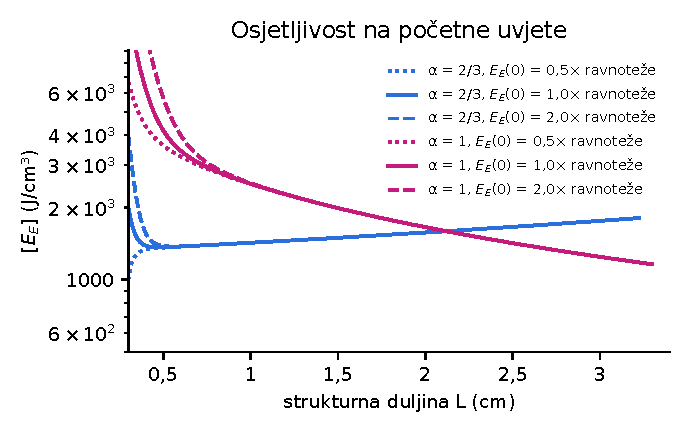
\includegraphics[width=0.66\linewidth]{figures/fig_pocetni_uvjeti.pdf}
\caption{Gustoća spremišta uz početno spremište od 0,5×, 1× i 2× ravnotežne vrijednosti, za $\alpha=2/3$ i $\alpha=1$ (početak pri $L_0=0{,}3$~cm).}
\label{fig:pu}
\end{figure}

Početno spremište postavljeno je na 0,5× ili 2× ravnotežne vrijednosti. Krivulje se ipak spajaju s referentnom (unutar 5~\%) već pri $L\approx\ICtwoThirdsLo$–$\ICtwoThirdsHi$~cm za $\alpha=2/3$, odnosno $L\approx\IConeLo$–$\IConeHi$~cm za $\alpha=1$. Razlika između $\alpha=2/3$ i $\alpha=1$ dakle nije artefakt početnih uvjeta. Kvalitativni rezultat S1 (H7) je robustan, a početni uvjeti važni su samo za najmanje jedinke.

\subsection{S6 · Monte Carlo: koji podaci otkrivaju $\alpha$}

Za svaki dizajn podataka i istinski $\alpha\in\{0{,}75;\,0{,}90\}$ generirano je \MCreps{} sintetskih skupova. Na svaki je zatim fitano šest parametara ($\pAm$, $\pM$, $\beta_S$, $k_E$, $\beta_E$, $\alpha$), s $\alpha$ ograničenim na 0,5–1,2 i dvjema početnim vrijednostima ($\alpha_0\in\{0{,}70;\,0{,}95\}$); zadržan je fit s manjim zbrojem kvadrata reziduala. Gornja granica 1,2 namjerno je iznad 1, jer se radna granica $\alpha\le1$ iz H3 pri fitanju ne smije nametnuti.
\begin{itemize}
\item Duljina $L(t)$: 25 mjerenja od 20. do 1200. dana s 2~\% šuma.
\item Spremište $[E_E]$: log-normalni šum.
\item Gladovanje: tri skupine (gladovanje počinje 200., 600. i 1200. dana, tj. pri $L\approx1$, 2 i 3~cm), spremište izmjereno 0, 10, 20 i 40 dana nakon početka, s 15~\% šuma.
\item Dizajni označeni zvjezdicom: podaci generirani s $a=0{,}72$, a fit pretpostavlja $a=2/3$ (pogrešno zadan eksponent asimilacije).
\end{itemize}

\begin{table}[ht]
\centering\small
\caption{Rezultati Monte Carlo procjene $\alpha$ (\MCreps{} ponavljanja po retku). RMSE je korijen srednje kvadratne pogreške, a zadnji stupac je udio procjena unutar $\pm0{,}05$ od istine.}
\label{tab:mc}
\begin{tabularx}{\linewidth}{@{}lXcccc r@{}}
\toprule
 & Dizajn podataka & istina & medijan $\hat\alpha$ & 10.–90. perc. & RMSE & $|\hat\alpha-\alpha|\le0{,}05$ \\
\midrule
\inputtab figures/tables/tab_mc.tex
\bottomrule
\end{tabularx}
\end{table}

\begin{figure}[ht]
\centering
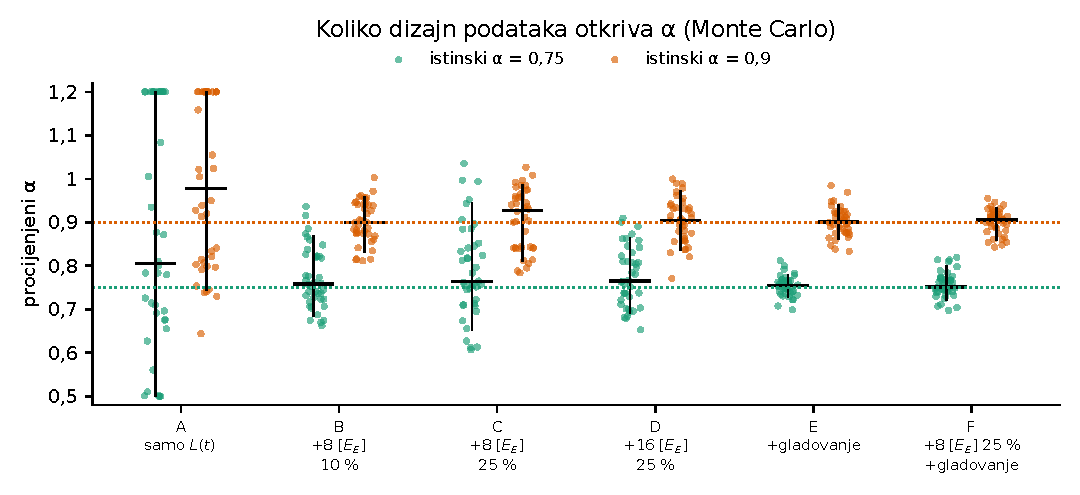
\includegraphics[width=\linewidth]{figures/fig_monte_carlo.pdf}
\caption{Procjene $\alpha$ po dizajnu podataka. Točke su pojedinačni fitovi, crne crte medijan i 10.–90. percentil, točkaste crte istinske vrijednosti. Prikazani su samo scenariji s ispravno zadanim $a$.}
\label{fig:mc}
\end{figure}

\textbf{Što pokazuje Monte Carlo:}
\begin{itemize}
\item \textbf{Samo $L(t)$ (A):} procjene se raspršuju po cijelom dopuštenom rasponu. Uz istinski $\alpha=0{,}75$ 10.–90. percentil je \MCAsevenfiveLo–\MCAsevenfiveHi, a 15–19 od \MCreps{} fitova po scenariju (37,5–47,5~\%) završi na granici raspona. RMSE je do \MCArmse. Iz samog rasta $\alpha$ nije identifikabilan; to je numerički izraz P4(i).
\item \textbf{Spremište (B–D)} smanjuje pogrešku. Uz 10~\% mjerne pogreške RMSE je do \MCBrmse{} (B), uz 25~\% do \MCCrmse{} s 8 točaka (C), odnosno do \MCDrmse{} sa 16 točaka (D). Lošija preciznost mjerenja nadoknađuje se većim brojem jedinki.
\item \textbf{Gladovanje (E) i kombinacija (F)} daju najmanju pogrešku: RMSE do \MCErmse{} (E) i \MCFrmse{} (F), uz barem 88~\% procjena unutar $\pm0{,}05$ od istine. Gladovanje je najbolji pojedinačni dizajn: nagib pražnjenja izravno daje $\alpha-1$ i ne ovisi o $a$ (P3).
\item \textbf{Pogrešno zadan $a$ pomiče $\hat\alpha$ prema dolje}, kako predviđa korolar P2: $\hat\alpha\approx\alpha-(a-2/3)=0{,}75-0{,}053\approx0{,}697$. Medijan dizajna C pada s \MCCokMed{} na \MCCmisMed, a dizajna F s \MCFokMed{} na \MCFmisMed; oba su unutar 0,012 od predviđanja. Pristranost ostaje i u dizajnu F, iako gladovanje samo po sebi ne ovisi o $a$, jer u zajedničkom fitu podaci o spremištu i rastu vuku procjenu prema pogrešnom $a$. Dizajn E s pogrešnim $a$ nije simuliran.
\item \textbf{Redoslijed za protokol:} najprije serija gladovanja u više veličina, zatim spremište po strukturi prema veličini, uz mjerenje unosa hrane prema veličini (eksponent $a$). Sam rast nikad nije dovoljan.
\end{itemize}

\begin{upozorenje}[Realnost]
Sintetski podaci su „najbolji slučaj“: nema varijabilnosti među jedinkama, a hrana i temperatura su poznate i stalne. Stvarni podaci dat će šire intervale. Rezultate treba čitati kao \emph{donju granicu} nesigurnosti i kao rangiranje dizajna, a ne kao očekivanu preciznost.
\end{upozorenje}

\begin{upozorenje}[Numerička lekcija iz ovog rada]
U prvoj verziji Monte Carla fit se zaustavljao nakon dvadesetak evaluacija, blizu početne vrijednosti $\alpha$. Uzrok je bio korak konačnih razlika za Jacobijevu matricu (zadano $\sim10^{-8}$), manji od tolerancije ODE rješavača ($10^{-7}$). Gradijent je zato bio šum, a „procjena“ je ostajala jednaka početnoj vrijednosti. Rješenje: relativni korak $10^{-3}$, više početnih vrijednosti $\alpha$ i provjera broja evaluacija. Isto vrijedi za fitanje u AmP-u (DEBtool) ili u bilo kojem drugom okruženju.
\end{upozorenje}
